\documentclass[a4paper,11pt]{article}
\usepackage{fullpage}
\usepackage{standalone}
\usepackage[utf8]{inputenc}
\usepackage[british]{babel}
\usepackage{csquotes}
\usepackage[T1]{fontenc}
\usepackage{amsmath}
\usepackage{amssymb}
\usepackage{mathtools}
\usepackage{mathptmx}
\usepackage{natbib}
\usepackage[final,babel]{microtype}
\usepackage[colorlinks,linkcolor=blue,citecolor=blue,urlcolor=blue]{hyperref}
\usepackage{doi}
\usepackage{siunitx}
\usepackage[margin=3pt]{subcaption}
\usepackage{xcolor}
\PassOptionsToPackage{final}{graphicx}
\usepackage{tikz}
\usetikzlibrary{arrows}
\usetikzlibrary{patterns}
\usepackage{bm}
\usepackage{booktabs}
\usepackage{tabularx}
\usepackage{enumitem}
\usepackage{titlesec}
\usepackage{colortbl}

\title{
\vspace*{-2em}
Monitoring committee progress report \#6\\
\vspace*{1em}
\Large{Numerical representation of mountains in atmospheric models}}
\author{James Shaw
\vspace{0.5em} \\
\large{Supervisors: Hilary Weller, John Methven, Terry Davies}
\vspace{0.5em} \\
\large{Monitoring committee: Paul Williams, Maarten Ambaum}}
\date{December 2017}

\captionsetup{margin=3pt,font={small}}
\setlength{\bibsep}{0.3em plus 0.1ex}

\makeatletter
\AtBeginDocument{
  \hypersetup{
    pdftitle = {Monitoring Committee Progress Report \#6},
    pdfauthor = {James Shaw}
  }
}
\makeatother

% https://tex.stackexchange.com/q/139401/23339
\graphicspath{{src/mc-report-2017-12/}{build/}}

% https://tex.stackexchange.com/a/79060/23339
\makeatletter
\def\input@path{{src/mc-report-2017-12/}{build/mc-report-2017-12/}{build/}}
\makeatother

\definecolor{done}{rgb}{0.87,0.96,0.87}

\makeatletter
\patchcmd{\ttlh@hang}{\parindent\z@}{\parindent\z@\leavevmode}{}{}
\patchcmd{\ttlh@hang}{\noindent}{}{}{}
\makeatother

\newcommand{\iu}{{i\mkern1mu}}
\newcommand{\TODO}[1]{\textcolor{purple}{TODO: \emph{#1}}}
\newcommand{\isep}{\mathrel{{.}\,{.}}\nobreak}

\begin{document}
\maketitle

\section{Introduction}

\section{Generalising the Charney--Phillips staggering for arbitrary meshes}

\href{http://www.datumedge.co.uk/publications/mc-report-2017-06.pdf}{Monitoring committee report \#5} demonstrated results of a new test case designed to excite the Lorenz computational mode.  A fully-compressible Euler model included a newly-formulated generalisation of the Charney--Phillips staggering for arbitrary meshes.
Unlike the model with Lorenz staggering, the Lorenz computational mode was not present in the new Charney--Phillips model.
These results were obtained on a uniform mesh using a low-accuracy advective form scheme for transporting potential temperature.  We set out to design a more accurate transport scheme and perform tests using distorted meshes in order to exercise the generalised Charney--Phillips staggering more thoroughly.

\TODO{
\begin{itemize}
\item plot: arakawaKonor Lorenz and C--P results on horizontal edgeGraded mesh
\item plot: arakawaKonor energy conservation
\item plot: arakawaKonorAdvect tracer conservation
\end{itemize}
}

% however, I've been unable to concoct a more accurate transport scheme, and the low-accuracy scheme produces bad results on distorted meshes
% advective form is non-conservative and this has spoiled test results
% but not obvious how to formulate a flux-form scheme, and would require averaging of winds, too
% I'll write up what we've achieved so far in the thesis (but not into a paper)
% but I don't want to spend further time on C--P because it looks like a dead end
% instead, I want to pursue work on highOrderFit, which has already been successful in 1D

\section{High-order transport for arbitrary meshes}

The cubicFit transport scheme solves the transport equation by approximating fluxes through faces using a multidimensional polynomial reconstruction \citep{shaw2017}.
The reconstruction fits a polynomial over known values stored at cell centre points, and this point-wise approach limits the cubicFit scheme to second-order convergence.
\citet{devendran2017} have developed a high-order finite volume scheme for solving Poisson's equation, and we apply their approach to obtain a transport scheme with high-order convergence.
Since it has much in common with the cubicFit scheme, we name this high-order scheme `highOrderFit'. 

Instead of a point-wise reconstruction that uses cell centre positions, the highOrderFit scheme constrains the polynomial fit so that the average of the polynomial integrated over a cell volume equals the cell average value.
Applying this constraint to each cell in the reconstruction stencil produces an overdetermined linear system that is solved using a weighted least squares approach in a similar manner to the cubicFit scheme \citep{shaw2017}.
Since we use the same reconstruction stencil, the highOrderFit scheme has the same computational cost per time-stage as the cubicFit scheme.

\begin{figure}
	\centering
	\begin{tikzpicture}[
	  scale=0.53,
	  cpnt/.style={fill=gray},
	]
	\draw [->] (-5,0) -- (5.5,0) node [right] {$x$};
	\draw (-3,-0.5) -- (-3,0.5);
	\draw (-1,-0.5) -- (-1,0.5);
	\draw (1,-0.5) -- (1,0.5) node [above] {$\phi_L$};
	\draw (3,-0.5) -- (3,0.5) node [above] {$\phi_R$};

	\path [cpnt] (-4,0) circle [radius=0.1] node [below] {$\phi_{j-2}$};
	\path [cpnt] (-2,0) circle [radius=0.1] node [below] {$\phi_{j-1}$};
	\path [cpnt] (0,0) circle [radius=0.1] node [below] {$\phi_j$};
	\path [cpnt] (2,0) circle [radius=0.1] node [below] {$\phi_{j+1}$};
	\path [cpnt] (4,0) circle [radius=0.1] node [below] {$\phi_{j+2}$};
	\draw [thick] (1,0) circle [radius=0.15];
	\draw [thick] (3,0) circle [radius=0.15];
	\end{tikzpicture}
	\caption{One-dimensional fluxes through a cell $\phi_{j+1}$ using four-point upwind-biased stencils to approximate fluxes $\phi_L$ and $\phi_R$.}
	\label{fig:1d-stencil}
\end{figure}

In one dimension, the reconstruction stencil comprises three upwind cells and one downwind cell.
Every cell has a left and right face, each with its own four-point stencil (figure~\ref{fig:1d-stencil}).
Hence, assuming a suitably high-order time-stepping scheme, highOrderFit should achieve fourth-order convergence because the flux divergence is approximated with five points.

We verify that highOrderFit achieves fourth-order convergence using a simple one-dimensional transport test.  The periodic domain is defined over the interval $[0,1]$ with a uniform velocity field $u = 1$ and an initial tracer field $\phi$ being defined as
\begin{align}
	\phi(x) = \exp \left( -b \left( x - x_0 \right)^2 \right)
\end{align}
where the Gaussian hill is centred at $x_0 = 0.5$ with $b = 80$.

Since we are interested in achieving high-order convergence on arbitrary meshes, the one-dimensional domain is divided into $N$ unequal intervals such that $\Delta x_i, \: i = 1\isep N$ becomes gradually coarser with increasing $i$.  The nonuniform mesh is smooth except for a discontinuity between $\Delta x_1$ and $\Delta x_N$ at the periodic boundary.

\begin{figure}
	\centering
	% GNUPLOT: LaTeX picture with Postscript
\begingroup
  \makeatletter
  \providecommand\color[2][]{%
    \GenericError{(gnuplot) \space\space\space\@spaces}{%
      Package color not loaded in conjunction with
      terminal option `colourtext'%
    }{See the gnuplot documentation for explanation.%
    }{Either use 'blacktext' in gnuplot or load the package
      color.sty in LaTeX.}%
    \renewcommand\color[2][]{}%
  }%
  \providecommand\includegraphics[2][]{%
    \GenericError{(gnuplot) \space\space\space\@spaces}{%
      Package graphicx or graphics not loaded%
    }{See the gnuplot documentation for explanation.%
    }{The gnuplot epslatex terminal needs graphicx.sty or graphics.sty.}%
    \renewcommand\includegraphics[2][]{}%
  }%
  \providecommand\rotatebox[2]{#2}%
  \@ifundefined{ifGPcolor}{%
    \newif\ifGPcolor
    \GPcolortrue
  }{}%
  \@ifundefined{ifGPblacktext}{%
    \newif\ifGPblacktext
    \GPblacktexttrue
  }{}%
  % define a \g@addto@macro without @ in the name:
  \let\gplgaddtomacro\g@addto@macro
  % define empty templates for all commands taking text:
  \gdef\gplbacktext{}%
  \gdef\gplfronttext{}%
  \makeatother
  \ifGPblacktext
    % no textcolor at all
    \def\colorrgb#1{}%
    \def\colorgray#1{}%
  \else
    % gray or color?
    \ifGPcolor
      \def\colorrgb#1{\color[rgb]{#1}}%
      \def\colorgray#1{\color[gray]{#1}}%
      \expandafter\def\csname LTw\endcsname{\color{white}}%
      \expandafter\def\csname LTb\endcsname{\color{black}}%
      \expandafter\def\csname LTa\endcsname{\color{black}}%
      \expandafter\def\csname LT0\endcsname{\color[rgb]{1,0,0}}%
      \expandafter\def\csname LT1\endcsname{\color[rgb]{0,1,0}}%
      \expandafter\def\csname LT2\endcsname{\color[rgb]{0,0,1}}%
      \expandafter\def\csname LT3\endcsname{\color[rgb]{1,0,1}}%
      \expandafter\def\csname LT4\endcsname{\color[rgb]{0,1,1}}%
      \expandafter\def\csname LT5\endcsname{\color[rgb]{1,1,0}}%
      \expandafter\def\csname LT6\endcsname{\color[rgb]{0,0,0}}%
      \expandafter\def\csname LT7\endcsname{\color[rgb]{1,0.3,0}}%
      \expandafter\def\csname LT8\endcsname{\color[rgb]{0.5,0.5,0.5}}%
    \else
      % gray
      \def\colorrgb#1{\color{black}}%
      \def\colorgray#1{\color[gray]{#1}}%
      \expandafter\def\csname LTw\endcsname{\color{white}}%
      \expandafter\def\csname LTb\endcsname{\color{black}}%
      \expandafter\def\csname LTa\endcsname{\color{black}}%
      \expandafter\def\csname LT0\endcsname{\color{black}}%
      \expandafter\def\csname LT1\endcsname{\color{black}}%
      \expandafter\def\csname LT2\endcsname{\color{black}}%
      \expandafter\def\csname LT3\endcsname{\color{black}}%
      \expandafter\def\csname LT4\endcsname{\color{black}}%
      \expandafter\def\csname LT5\endcsname{\color{black}}%
      \expandafter\def\csname LT6\endcsname{\color{black}}%
      \expandafter\def\csname LT7\endcsname{\color{black}}%
      \expandafter\def\csname LT8\endcsname{\color{black}}%
    \fi
  \fi
    \setlength{\unitlength}{0.0500bp}%
    \ifx\gptboxheight\undefined%
      \newlength{\gptboxheight}%
      \newlength{\gptboxwidth}%
      \newsavebox{\gptboxtext}%
    \fi%
    \setlength{\fboxrule}{0.5pt}%
    \setlength{\fboxsep}{1pt}%
\begin{picture}(5040.00,2880.00)%
    \gplgaddtomacro\gplbacktext{%
      \csname LTb\endcsname%
      \put(726,704){\makebox(0,0)[r]{\strut{}$-0.2$}}%
      \put(726,977){\makebox(0,0)[r]{\strut{}$0$}}%
      \put(726,1250){\makebox(0,0)[r]{\strut{}$0.2$}}%
      \put(726,1523){\makebox(0,0)[r]{\strut{}$0.4$}}%
      \put(726,1796){\makebox(0,0)[r]{\strut{}$0.6$}}%
      \put(726,2069){\makebox(0,0)[r]{\strut{}$0.8$}}%
      \put(726,2342){\makebox(0,0)[r]{\strut{}$1$}}%
      \put(726,2615){\makebox(0,0)[r]{\strut{}$1.2$}}%
      \put(858,484){\makebox(0,0){\strut{}$0$}}%
      \put(1237,484){\makebox(0,0){\strut{}$0.1$}}%
      \put(1615,484){\makebox(0,0){\strut{}$0.2$}}%
      \put(1994,484){\makebox(0,0){\strut{}$0.3$}}%
      \put(2372,484){\makebox(0,0){\strut{}$0.4$}}%
      \put(2751,484){\makebox(0,0){\strut{}$0.5$}}%
      \put(3129,484){\makebox(0,0){\strut{}$0.6$}}%
      \put(3508,484){\makebox(0,0){\strut{}$0.7$}}%
      \put(3886,484){\makebox(0,0){\strut{}$0.8$}}%
      \put(4265,484){\makebox(0,0){\strut{}$0.9$}}%
      \put(4643,484){\makebox(0,0){\strut{}$1$}}%
    }%
    \gplgaddtomacro\gplfronttext{%
      \csname LTb\endcsname%
      \put(220,1659){\rotatebox{-270}{\makebox(0,0){\strut{}$\phi$}}}%
      \put(2750,154){\makebox(0,0){\strut{}$x$}}%
      \csname LTb\endcsname%
      \put(3656,2442){\makebox(0,0)[r]{\strut{}Initial}}%
      \csname LTb\endcsname%
      \put(3656,2222){\makebox(0,0)[r]{\strut{}Final}}%
    }%
    \gplbacktext
    \put(0,0){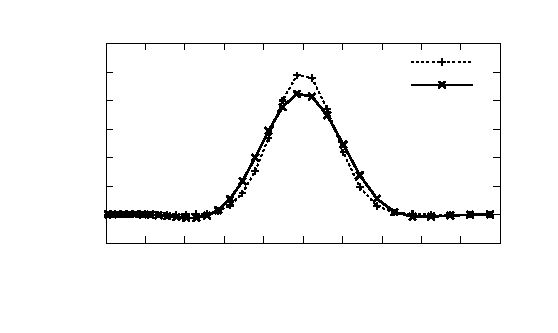
\includegraphics{tracer}}%
    \gplfronttext
  \end{picture}%
\endgroup

	\caption{One-dimensional transport of a Gaussian hill across a periodic domain using the highOrderFit scheme.  The initial tracer is transported in a uniform velocity field exactly once around the domain so that the analytic solution is equal to the initial solution marked by a dotted line.  The numerical solution is marked by a solid line and cell centre averages are marked by crosses.}
	\label{fig:advect1D-tracer}
\end{figure}

The test is integrated forward by one time unit such that the tracer is transported exactly once around the periodic domain such that the analytic solution is equal to the initial solution.  A solution on a rather coarse mesh with $N = 32$ is illustrated in figure~\ref{fig:advect1D-tracer} with the initial solution marked by a dotted line and the final numerical solution marked by a solid line, with cell centre averages marked by crosses.

\begin{figure}
	\centering
	% GNUPLOT: LaTeX picture with Postscript
\begingroup
  \makeatletter
  \providecommand\color[2][]{%
    \GenericError{(gnuplot) \space\space\space\@spaces}{%
      Package color not loaded in conjunction with
      terminal option `colourtext'%
    }{See the gnuplot documentation for explanation.%
    }{Either use 'blacktext' in gnuplot or load the package
      color.sty in LaTeX.}%
    \renewcommand\color[2][]{}%
  }%
  \providecommand\includegraphics[2][]{%
    \GenericError{(gnuplot) \space\space\space\@spaces}{%
      Package graphicx or graphics not loaded%
    }{See the gnuplot documentation for explanation.%
    }{The gnuplot epslatex terminal needs graphicx.sty or graphics.sty.}%
    \renewcommand\includegraphics[2][]{}%
  }%
  \providecommand\rotatebox[2]{#2}%
  \@ifundefined{ifGPcolor}{%
    \newif\ifGPcolor
    \GPcolortrue
  }{}%
  \@ifundefined{ifGPblacktext}{%
    \newif\ifGPblacktext
    \GPblacktexttrue
  }{}%
  % define a \g@addto@macro without @ in the name:
  \let\gplgaddtomacro\g@addto@macro
  % define empty templates for all commands taking text:
  \gdef\gplbacktext{}%
  \gdef\gplfronttext{}%
  \makeatother
  \ifGPblacktext
    % no textcolor at all
    \def\colorrgb#1{}%
    \def\colorgray#1{}%
  \else
    % gray or color?
    \ifGPcolor
      \def\colorrgb#1{\color[rgb]{#1}}%
      \def\colorgray#1{\color[gray]{#1}}%
      \expandafter\def\csname LTw\endcsname{\color{white}}%
      \expandafter\def\csname LTb\endcsname{\color{black}}%
      \expandafter\def\csname LTa\endcsname{\color{black}}%
      \expandafter\def\csname LT0\endcsname{\color[rgb]{1,0,0}}%
      \expandafter\def\csname LT1\endcsname{\color[rgb]{0,1,0}}%
      \expandafter\def\csname LT2\endcsname{\color[rgb]{0,0,1}}%
      \expandafter\def\csname LT3\endcsname{\color[rgb]{1,0,1}}%
      \expandafter\def\csname LT4\endcsname{\color[rgb]{0,1,1}}%
      \expandafter\def\csname LT5\endcsname{\color[rgb]{1,1,0}}%
      \expandafter\def\csname LT6\endcsname{\color[rgb]{0,0,0}}%
      \expandafter\def\csname LT7\endcsname{\color[rgb]{1,0.3,0}}%
      \expandafter\def\csname LT8\endcsname{\color[rgb]{0.5,0.5,0.5}}%
    \else
      % gray
      \def\colorrgb#1{\color{black}}%
      \def\colorgray#1{\color[gray]{#1}}%
      \expandafter\def\csname LTw\endcsname{\color{white}}%
      \expandafter\def\csname LTb\endcsname{\color{black}}%
      \expandafter\def\csname LTa\endcsname{\color{black}}%
      \expandafter\def\csname LT0\endcsname{\color{black}}%
      \expandafter\def\csname LT1\endcsname{\color{black}}%
      \expandafter\def\csname LT2\endcsname{\color{black}}%
      \expandafter\def\csname LT3\endcsname{\color{black}}%
      \expandafter\def\csname LT4\endcsname{\color{black}}%
      \expandafter\def\csname LT5\endcsname{\color{black}}%
      \expandafter\def\csname LT6\endcsname{\color{black}}%
      \expandafter\def\csname LT7\endcsname{\color{black}}%
      \expandafter\def\csname LT8\endcsname{\color{black}}%
    \fi
  \fi
    \setlength{\unitlength}{0.0500bp}%
    \ifx\gptboxheight\undefined%
      \newlength{\gptboxheight}%
      \newlength{\gptboxwidth}%
      \newsavebox{\gptboxtext}%
    \fi%
    \setlength{\fboxrule}{0.5pt}%
    \setlength{\fboxsep}{1pt}%
\begin{picture}(7200.00,3600.00)%
    \gplgaddtomacro\gplbacktext{%
      \csname LTb\endcsname%
      \put(588,648){\makebox(0,0)[r]{\strut{}$10^{-7}$}}%
      \put(588,981){\makebox(0,0)[r]{\strut{}$10^{-6}$}}%
      \put(588,1314){\makebox(0,0)[r]{\strut{}$10^{-5}$}}%
      \put(588,1647){\makebox(0,0)[r]{\strut{}$10^{-4}$}}%
      \put(588,1980){\makebox(0,0)[r]{\strut{}$10^{-3}$}}%
      \put(588,2313){\makebox(0,0)[r]{\strut{}$10^{-2}$}}%
      \put(588,2646){\makebox(0,0)[r]{\strut{}$10^{-1}$}}%
      \put(720,428){\makebox(0,0){\strut{}$10^{-3}$}}%
      \put(1979,428){\makebox(0,0){\strut{}$10^{-2}$}}%
      \put(3239,428){\makebox(0,0){\strut{}$10^{-1}$}}%
    }%
    \gplgaddtomacro\gplfronttext{%
      \csname LTb\endcsname%
      \put(-23,1763){\rotatebox{-270}{\makebox(0,0){\strut{}$\ell_2$ error}}}%
      \put(1979,98){\makebox(0,0){\strut{}$\max(\Delta x)$}}%
      \csname LTb\endcsname%
      \put(2384,3427){\makebox(0,0)[r]{\strut{}cubicFit}}%
      \csname LTb\endcsname%
      \put(2384,3207){\makebox(0,0)[r]{\strut{}highOrderFit}}%
    }%
    \gplgaddtomacro\gplbacktext{%
      \csname LTb\endcsname%
      \put(4188,648){\makebox(0,0)[r]{\strut{}$10^{-7}$}}%
      \put(4188,981){\makebox(0,0)[r]{\strut{}$10^{-6}$}}%
      \put(4188,1314){\makebox(0,0)[r]{\strut{}$10^{-5}$}}%
      \put(4188,1647){\makebox(0,0)[r]{\strut{}$10^{-4}$}}%
      \put(4188,1980){\makebox(0,0)[r]{\strut{}$10^{-3}$}}%
      \put(4188,2313){\makebox(0,0)[r]{\strut{}$10^{-2}$}}%
      \put(4188,2646){\makebox(0,0)[r]{\strut{}$10^{-1}$}}%
      \put(4320,428){\makebox(0,0){\strut{}$10^{-3}$}}%
      \put(5580,428){\makebox(0,0){\strut{}$10^{-2}$}}%
      \put(6839,428){\makebox(0,0){\strut{}$10^{-1}$}}%
    }%
    \gplgaddtomacro\gplfronttext{%
      \csname LTb\endcsname%
      \put(3577,1763){\rotatebox{-270}{\makebox(0,0){\strut{}$\ell_\infty$ error}}}%
      \put(5579,98){\makebox(0,0){\strut{}$\max(\Delta x)$}}%
      \csname LTb\endcsname%
      \put(5984,3427){\makebox(0,0)[r]{\strut{}$x^2$}}%
      \csname LTb\endcsname%
      \put(5984,3207){\makebox(0,0)[r]{\strut{}$x^4$}}%
    }%
    \gplbacktext
    \put(0,0){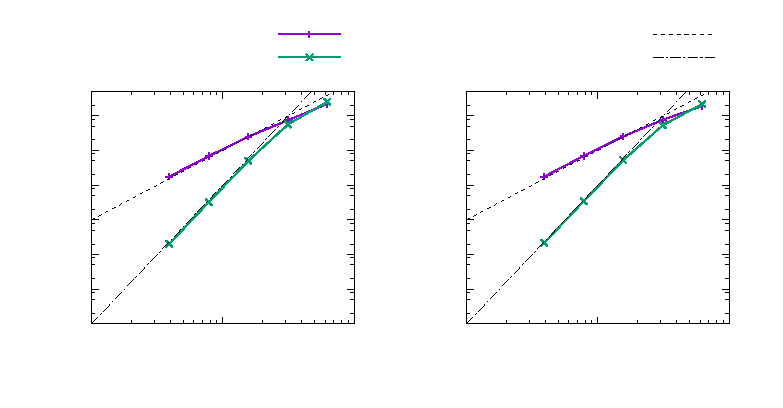
\includegraphics{convergence}}%
    \gplfronttext
  \end{picture}%
\endgroup

	\caption{Convergence of the cubicFit and highOrderFit schemes in the one-dimensional transport test.
	The error norms are defined as $\ell_2 = \left( \sum \left( \left( \phi - \phi_T \right)^2 \Delta x \right) / \sum \left( \phi_T^2 \Delta x \right)\right)^{1/2}$ and $\ell_\infty = \max \left| \phi - \phi_T \right| / \max \left| \phi_T \right|$ where $\phi$ is the numerical solution and $\phi_T$ is the analytic solution.}
	\label{fig:advect1D-convergence}
\end{figure}

Convergence tests are performed comparing cubicFit and highOrderFit transport schemes using meshes with cell counts between $N = 2^4$ and $N = 2^8$.  The classical fourth-order Runge--Kutta time-stepping scheme \citep[p. 53]{durran2013} is used for both transport schemes.  The cubicFit scheme is limited to second-order convergence while the highOrderFit scheme is fourth-order convergent (figure~\ref{fig:advect1D-convergence}).

\section{Future research}

% Generalisation of Charney--Phillips staggering not going so well
% but high-order transport scheme going much better

\section{Personal development}

I continue to give regular talks at group meetings and I have arranged to give a lunchtime seminar in January 2018.
I have also been invited by \href{http://staff.southwales.ac.uk/users/8005-jkent}{James Kent} to speak at a mathematics departmental seminar at University of South Wales where Dr Kent lectures.

I also continue searching for postdoctoral vacancies.
I was unsuccessful in my application for a Mozilla science fellowship, though I was very happy to be placed amongst the top 5\% of more than 1000 applicants.
I was offered a position as a scientific software engineer at the Met Office, but chose to decline since the role was focused on software development with few opportunities for scientific research.
I was also interviewed for a postdoctoral position developing numerical methods for flood forecasts at the University of Sheffield, but the position was given to a more experienced candidate.

I have worked with David Dritschel at the University of St Andrews and Alan Blyth, Doug Parker and Steven B\"{o}ing at the University of Leeds to submit an EPSRC proposal that extends the Moist Parcel-in-a-Cell model \citep{boeing2017} for studying cloud turbulence.  We expect the EPSRC to reach a decision around March 2018.
I am also a named postdoctoral researcher on a NERC proposal to study physics-dynamics coupling that Hilary submitted in collaboration with Jemma Shipton, Colin Cotter, Peter Clark and John Thuburn in July 2017.
\TODO{what happens next to the NERC proposal?}
I continue to monitor job boards for new vacancies.

\bibliographystyle{ametsoc2014}                                                 
\bibliography{src/mc-report-2017-12/references}

\newpage

\titlespacing\subsubsection{0pt}{0.8em plus 4pt minus 2pt}{0.2em plus 2pt minus 2pt}

\section*{Appendix A: Thesis plan}
\footnotesize
A work-in-progress draft is available at \url{http://www.datumedge.co.uk/publications/phd-thesis.pdf}.

\subsubsection*{1. Introduction}
\begin{tabularx}{\linewidth}{>{\hsize=0.9in}X X}
Not started & This project is motivated by the need for alternative horizontal and vertical representations of Earth's atmosphere in the proximity to mountainous terrain
\end{tabularx}

\subsubsection*{2. Numerically stable transport over steep slopes}
\noindent The cubicFit transport scheme is stable and accurate over steep slopes with arbitrary, distorted meshes.
\vspace*{0.5em}

\begin{tabularx}{\linewidth}{>{\hsize=0.9in}X X}
\rowcolor{done}	Complete & Review of existing transport schemes and motivation for the cubicFit transport scheme \\
\rowcolor{done}	Complete & Document the cubicFit transport scheme \\
\addlinespace[0.5em]
	 & Test results comparing a standard linear upwind scheme and the cubicFit transport scheme: \\
\rowcolor{done}	Complete & \quad\textbullet\enspace horizontal transport test above steep slopes \\
\rowcolor{done}	Complete & \quad\textbullet\enspace terrain-following transport test above steep slopes \\
\rowcolor{done} Complete & \quad\textbullet\enspace deformational transport tests on a spherical Earth \\
\end{tabularx}

\subsubsection*{3. High-order transport for arbitrary meshes}
\noindent The cubicFit transport scheme is limited to second-order convergence because it uses a point-wise reconstruction of cell centre values.  If instead the reconstruction uses cell centre volume averages then higher-order convergence is achievable.
\vspace*{0.5em}

\begin{tabularx}{\linewidth}{>{\hsize=0.9in}X X}
Not started & Document the high-order transport scheme \\
\addlinespace[0.5em]
	 & Test results comparing cubicFit and highOrderFit transport schemes: \\
Not started & \quad\textbullet\enspace two-dimensional solid body rotation of a Gaussian tracer on distorted meshes \citep{chen2017} \\
Not started & \quad\textbullet\enspace horizontal transport of a cosine bell tracer above steep slopes as in chapter 2
\end{tabularx}

\subsubsection*{4. A new mesh for representing the atmosphere above terrain}
\noindent The slanted cell mesh reduces errors associated with pressure gradient calculations and avoids severe time-step constraints.
\vspace*{0.5em}

\begin{tabularx}{\linewidth}{>{\hsize=0.9in}X X}
\rowcolor{done} Complete & Introduction to pressure gradient calculations and existing methods to reduce errors associated with pressure gradient calculations \\
\rowcolor{done} Complete & Describe the new slanted cell method \\
\rowcolor{done} Complete & Transport test over a mountainous lower boundary using terrain-following, cut cell and slanted cell meshes \\
\rowcolor{done} Complete & A two-dimensional test of a quiescent atmosphere above steep slopes, comparing terrain-following, cut cell and slanted cell meshes \\
\end{tabularx}

\subsubsection*{5. Generalising the Charney--Phillips staggering for arbitrary meshes}
\noindent The Charney--Phillips staggering avoids the Lorenz computational mode, but it has only been formulated for structured quadrilateral meshes.  A generalised formulation will be suitable for arbitrary meshes.
\vspace*{0.5em}

\begin{tabularx}{\linewidth}{>{\hsize=1.3in}X X}
	In development & Describe the generalised Charney--Phillips formulation \\
	In development & Document the necessary changes to the nonhydrostatic model including the advective-form transport scheme \\
	In development & Compare the Charney--Phillips model variant with the Lorenz model using a standard mountain waves test case \citep{schaer2002} \\
	Not started & Document the new two-dimensional standing waves test case \\
	In development & Compare standing waves test results using Lorenz and Charney--Phillips model variants on a uniform mesh and rectangular meshes with sloping faces
\end{tabularx}

\subsubsection*{6. Discussion}
\vspace*{0.5em}

\begin{tabularx}{\linewidth}{>{\hsize=0.9in}X X}
Not started & 
\end{tabularx}


\newpage

\section*{Appendix B: Training record}

\subsubsection*{Mathematics modules}
\begin{tabular}{l l l l}
Spring 2017	& \href{https://finite-element.github.io}{M5A47}  & Finite elements: numerical analysis and implementation & unassessed, partially completed \\
Spring 2016	& \href{www.reading.ac.uk/module/document.aspx?modP=MA3NAT&modYR=1516}{MA3NAT} & Numerical Analysis II & unassessed \\
Spring 2015	& \href{www.reading.ac.uk/modules/document.aspx?modP=MAMNSP&modYR=1415}{MAMNSP} & Numerical Solution of Partial Differential Equations  & 78\% \\
\end{tabular}

\subsubsection*{RRDP modules}
I have completed the requisite 11 RRDP modules.

\vspace*{0.5em}
\begin{tabular}{l l}
23 June 2017    & Graduate school conference \\
3 May 2017	& Effective CVs \\
28 Feb 2017	& Getting your first post-doc position \\
9 Nov 2016      & Open Access and research data management \\
24 Mar 2016	& Voice coaching: looking after your voice \\
26--27 Jan 2016 & Preparing to teach (introduction, marking \& feedback, leading small groups) \\
2 Dec 2015	& An essential guide to critical academic writing \\
17 Nov 2015	& Understanding the UK higher education context \\
19 May 2015	& How to avoid plagiarism \\
10 Mar 2015	& How to write a literature review \\
19 Feb 2015	& How to write a paper \\
\end{tabular}

\subsubsection*{External courses}
\begin{tabular}{l l}
June 2016 & Dynamical core intercomparison project summer school, NCAR \\
13 May 2016 & Peer review: the nuts and bolts, Sense about Science \\
June 2015 & Advanced numerical methods for Earth-system modelling, ECMWF \\
\end{tabular}

\subsubsection*{Conferences and workshops}
\begin{tabularx}{\linewidth}{l l X}
September 2017 & Speaker & \href{https://sites.google.com/site/scicade2017/}{International conference on scientific computation and differential equations}, University of Bath \\
August 2017 & Co-organiser & \href{https://frontiers2017.wordpress.com/}{Frontiers in natural environment research}, Imperial College London \\
July 2017 & Speaker & Met Office GungHo network meeting, University of Exeter \\
June 2017 & Participant & \href{https://www.software.ac.uk/c4rr}{Docker containers for reproducible research}, University of Cambridge \\
April 2017 & Speaker & \href{https://forge.ipsl.jussieu.fr/heat/wiki/PDEs2017}{PDEs on the Sphere}, École normale supérieure, Paris \\
March 2017 & Attendee & \href{https://blogs.reading.ac.uk/open-research/open-in-practice-inspirations-strategies-and-methods-for-open-research/}{Open in practice: inspirations, strategies and methods for open research}, University of Reading \\
March 2017 & Participant & \href{http://www.effective-quadratures.org/eq2017}{Effective quadratures workshop}, University of Cambridge \\
February 2017 & Invited speaker & Numerical methods for geophysical fluid dynamics, Imperial College London \\
January 2017 & Attendee & Research software management, sharing and sustainability, British Library \\
December 2016 & Invited speaker & \href{https://www.rmets.org/events/meteorological-research-within-university-reading-2016}{South-East local centre meeting, Royal Meteorological Society} \\
October 2016 & Speaker & \href{http://www.ecmwf.int/en/learning/workshops-and-seminars/workshop-numerical-and-computational-methods-simulation-all-scale-geophysical-flows}{Numerical and computational methods for simulation of all-scale geophysical flows}, ECMWF \\
November 2015 & Attendee & GungHo workshop on next generation weather and climate prediction, Met Office \\
June 2015 & Attendee & Hoskins@70 \\
June 2015 & Poster & SCENARIO DTP conference \\
March 2015 & Speaker & \href{http://www.icms.org.uk/workshop.php?id=334}{Galerkin methods with applications in weather and climate forecasting}, ICMS \\
\end{tabularx}

\subsubsection*{Teaching}
\begin{tabular}{l l l}
Oct 2016 & Teaching assistant & MTMW11 fluid dynamics \\
Oct 2015 & Teaching assistant & MTMG02 atmospheric physics \\
Sep 2015 & Teaching assistant & NCAS summer school \\
Sep 2014 & Course teacher & MPE python and linux short course \\
\end{tabular}

\subsubsection*{Visits and collaborations}
\begin{tabularx}{\linewidth}{l X}
July 2016 & Organised visit from \href{https://www.youtube.com/user/SimonOxfPhys}{Simon Clark}, stratospheric PhD researcher and YouTube vlogger \\
Summer 2016 & Worked with Hilary's MSc student, Christiana Skea, studying variable time-stepping for ODEs \\
June 2016 & Visited NCAR, hosted by \href{http://www.image.ucar.edu/staff/rnair/}{Ram Nair} \\
2015 -- 2017 & Coauthoring an article about dimensionally-split and multidimensional transport schemes, written with Hilary, her former student \href{https://www.clisap.de/research/a:-climate-dynamics-and-variability/crg-numerical-methods-in-geosciences/team-members/yumeng-chen/}{Yumeng Chen}, and Stephen Pring at the Met Office \\
\end{tabularx}

\subsubsection*{Outreach}
\begin{tabular}{l l l}
17 Mar 2017 & ``\href{https://thesocialmetwork.wordpress.com/2017/03/17/simulating-wind-on-computers/}{The advection process: simulating wind on computers}'', Social Metwork blog article \\
14 Jul 2015 & Schools physicist of the year awards \\
14 Jun 2015 & East Reading festival \\
15 Feb 2015 & Brighton science festival \\
\end{tabular}

\subsubsection*{Presentations}
\begin{tabularx}{\linewidth}{l l X}
2 Feb 2018 & University of South Wales \\
22 Jan 2018 & HHH group \\
16 Jan 2018 & Lunchtime seminar \\
26 Oct 2017 & Comp. Atmos. Dyn. group & High-order finite volume advection \\
17 Oct 2017 & Mesoscale group & Numerical advection of chemical species \\
27 Sep 2017 & DARC group & Subsampling for uncertainty quantification \\
6 Jul 2017 & Comp. Atmos. Dyn. group & Charney--Phillips review and automated testing for OpenFOAM applications \\
19 Jun 2017 & HHH group & Subsampling for uncertainty quantification \\
17 Nov 2016 & Comp. Atmos. Dyn. group & A review of atmospheric transport schemes \\
9 Nov 2016 & PhD group & Replicable computational atmospheric science \\
31 Oct 2016 & HHH group & Advection over steep slopes \\
22 Sep 2016 & PhD poster session & Improving numerical accuracy over steep slopes \\
23 Mar 2016 & Quo Vadis & Numerical representation of orography in dynamical cores (honourable mention) \\
17 Feb 2016 & PhD group & Multidimensional advection schemes for arbitrary meshes \\
9 Feb 2016 & Mesoscale group & Curl-free pressure gradients for accurate modelling of cold air pools \\
19 Oct 2015 & HHH group & Improving modelled mountain flows with alternative representations of terrain \\
27 Apr 2015 & HHH group & A like-for-like comparison between terrain following and cut cell grids \\
21 Apr 2015 & PhD group & Discrete vector calculus on Arakawa C grids \\
12 Feb 2015 & Met Office & Poster presentation for Met Office Academic Partnership \\
18 Jan 2015 & PhD group & Python and linux tips \\
17 Dec 2014 & MPECDT jamboree & Poster presentation for Mathematics for Planet Earth Centre for Doctoral Training jamboree \\
12 Sep 2014 & Lunchtime seminar  & Gain control of your documents and code: hands-on with revision control and build automation \\
\end{tabularx}

\section*{Appendix C: Publication milestones}

\begin{tabular}{l l}
10 Jun 2015 & First MWR manuscript submitted \\
19 Aug 2015 & Major revisions required to MWR manuscript \\
29 Oct 2015 & Second MWR manuscript submitted\\
9 Dec 2015 & Major revisions required to MWR manuscript \\
5 Feb 2016 & Third MWR manuscript submitted
	\vspace*{1em} \\
2 Feb 2017 & First JCP manuscript submitted \\
13 Mar 2017 & Minor revisions required to JCP manuscript \\
21 Apr 2017 & Second JCP manuscript submitted \\
\end{tabular}

\end{document}
